%!TeX root=../pridetop.tex
\chapter[Chapter \thechapter]{}
	
	\begin{figure}[t!]
\centering
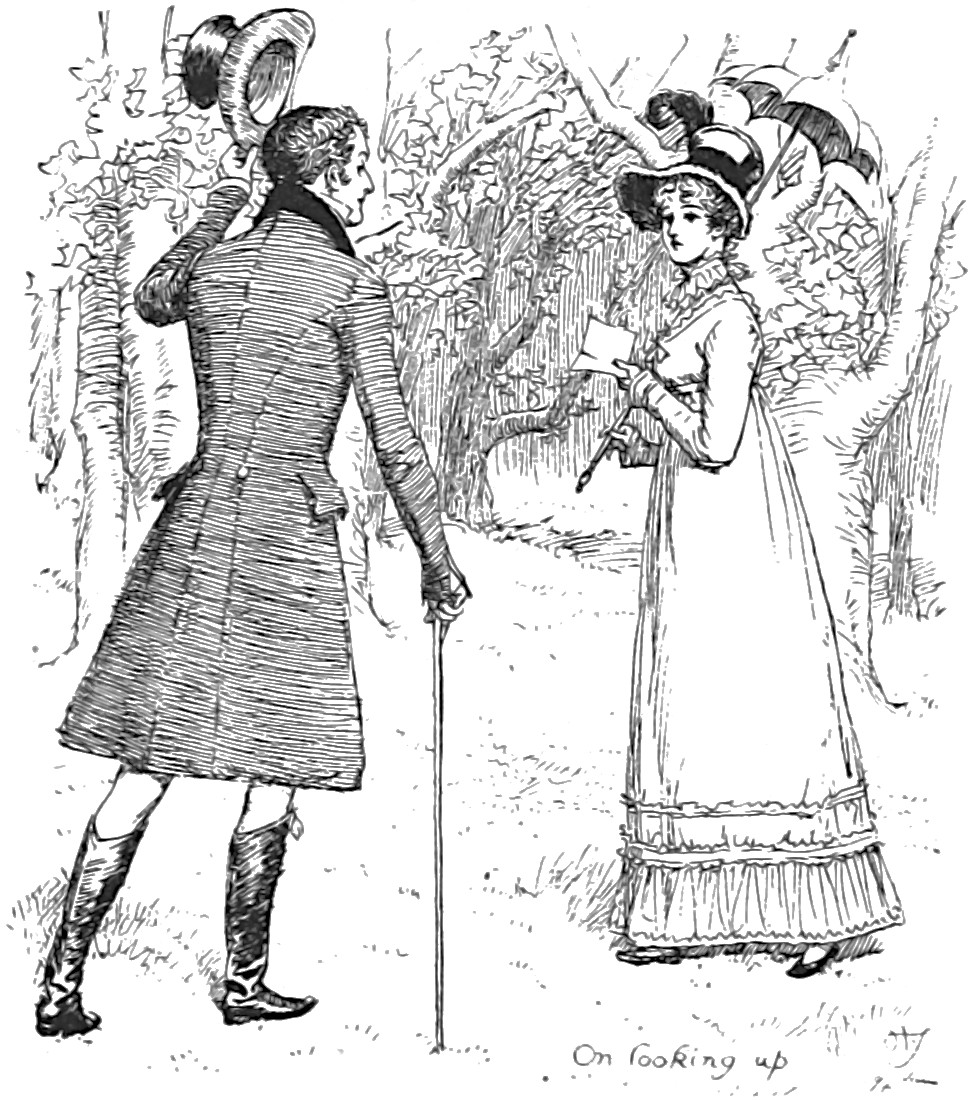
\includegraphics[width=.8\linewidth]{33top}
\captionlistentry{Headpiece to Chapter \thechapter}
\end{figure}


\lettrine[lines=6,image=true]{initials/chap33m}{ore}  than once did Elizabeth, in her ramble within the park, unexpectedly meet Mr Darcy. She felt all the perverseness of the mischance that should bring him where no one else was brought; and, to prevent its ever happening again, took care to inform him, at first, that it was a favourite haunt of hers. How it could occur a second time, therefore, was very odd! Yet it did, and even the third. It seemed like wilful ill-nature, or a voluntary penance; for on these occasions it was not merely a few formal inquiries and an awkward pause and then away, but he actually thought it necessary to turn back and walk with her. He never said a great deal, nor did she give herself the trouble of talking or of listening much; but it struck her in the course of their third rencounter that he was asking some odd unconnected questions—about her pleasure in being at Hunsford, her love of solitary walks, and her opinion of Mr and Mrs Collins's happiness; and that in speaking of Rosings, and her not perfectly understanding the house, he seemed to expect that whenever she came into Kent again she would be staying \textit{there} too. His words seemed to imply it. Could he have Colonel Fitzwilliam in his thoughts? She supposed, if he meant anything, he must mean an allusion to what might arise in that quarter. It distressed her a little, and she was quite glad to find herself at the gate in the pales opposite the Parsonage.

She was engaged one day, as she walked, in re-perusing Jane's last letter, and dwelling on some passages which proved that Jane had not written in spirits, when, instead of being again surprised by Mr Darcy, she saw, on looking up, that Colonel Fitzwilliam was meeting her. Putting away the letter immediately, and forcing a smile, she said,—

<I did not know before that you ever walked this way.>

<I have been making the tour of the park,> he replied, <as I generally do every year, and intended to close it with a call at the Parsonage. Are you going much farther?>

<No, I should have turned in a moment.>

And accordingly she did turn, and they walked towards the Parsonage together.

<Do you certainly leave Kent on Saturday?> said she.

<Yes—if Darcy does not put it off again. But I am at his disposal. He arranges the business just as he pleases.>

<And if not able to please himself in the arrangement, he has at least great pleasure in the power of choice. I do not know anybody who seems more to enjoy the power of doing what he likes than Mr Darcy.>

<He likes to have his own way very well,> replied Colonel Fitzwilliam. <But so we all do. It is only that he has better means of having it than many others, because he is rich, and many others are poor. I speak feelingly. A younger son, you know, must be inured to self-denial and dependence.>

<In my opinion, the younger son of an earl can know very little of either. Now, seriously, what have you ever known of self-denial and dependence? When have you been prevented by want of money from going wherever you chose or procuring anything you had a fancy for?>

<These are home questions—and perhaps I cannot say that I have experienced many hardships of that nature. But in matters of greater weight, I may suffer from the want of money. Younger sons cannot marry where they like.>

<Unless where they like women of fortune, which I think they very often do.>

<Our habits of expense make us too dependent, and there are not many in my rank of life who can afford to marry without some attention to money.>

<Is this,> thought Elizabeth, <meant for me?> and she coloured at the idea; but, recovering herself, said in a lively tone, <And pray, what is the usual price of an earl's younger son? Unless the elder brother is very sickly, I suppose you would not ask above fifty thousand pounds.>

He answered her in the same style, and the subject dropped. To interrupt a silence which might make him fancy her affected with what had passed, she soon afterwards said,—

<I imagine your cousin brought you down with him chiefly for the sake of having somebody at his disposal. I wonder he does not marry, to secure a lasting convenience of that kind. But, perhaps, his sister does as well for the present; and, as she is under his sole care, he may do what he likes with her.>

<No,> said Colonel Fitzwilliam, <that is an advantage which he must divide with me. I am joined with him in the guardianship of Miss Darcy.>

<Are you, indeed? And pray what sort of a guardian do you make? Does your charge give you much trouble? Young ladies of her age are sometimes a little difficult to manage; and if she has the true Darcy spirit, she may like to have her own way.>

As she spoke, she observed him looking at her earnestly; and the manner in which he immediately asked her why she supposed Miss Darcy likely to give them any uneasiness, convinced her that she had somehow or other got pretty near the truth. She directly replied,—

<You need not be frightened. I never heard any harm of her; and I dare say she is one of the most tractable creatures in the world. She is a very great favourite with some ladies of my acquaintance, Mrs Hurst and Miss Bingley. I think I have heard you say that you know them.>

<I know them a little. Their brother is a pleasant, gentlemanlike man—he is a great friend of Darcy's.>

<Oh yes,> said Elizabeth drily—<Mr Darcy is uncommonly kind to Mr Bingley, and takes a prodigious deal of care of him.>

<Care of him! Yes, I really believe Darcy \textit{does} take care of him in those points where he most wants care. From something that he told me in our journey hither, I have reason to think Bingley very much indebted to him. But I ought to beg his pardon, for I have no right to suppose that Bingley was the person meant. It was all conjecture.>

<What is it you mean?>

<It is a circumstance which Darcy of course could not wish to be generally known, because if it were to get round to the lady's family it would be an unpleasant thing.>

<You may depend upon my not mentioning it.>

<And remember that I have not much reason for supposing it to be Bingley. What he told me was merely this: that he congratulated himself on having lately saved a friend from the inconveniences of a most imprudent marriage, but without mentioning names or any other particulars; and I only suspected it to be Bingley from believing him the kind of young man to get into a scrape of that sort, and from knowing them to have been together the whole of last summer.>

<Did Mr Darcy give you his reasons for this interference?>

<I understood that there were some very strong objections against the lady.>

<And what arts did he use to separate them?>

<He did not talk to me of his own arts,> said Fitzwilliam, smiling. <He only told me what I have now told you.>

Elizabeth made no answer, and walked on, her heart swelling with indignation. After watching her a little, Fitzwilliam asked her why she was so thoughtful.

<I am thinking of what you have been telling me,> said she. <Your cousin's conduct does not suit my feelings. Why was he to be the judge?>

<You are rather disposed to call his interference officious?>

<I do not see what right Mr Darcy had to decide on the propriety of his friend's inclination; or why, upon his own judgment alone, he was to determine and direct in what manner that friend was to be happy. But,> she continued, recollecting herself, <as we know none of the particulars, it is not fair to condemn him. It is not to be supposed that there was much affection in the case.>

<That is not an unnatural surmise,> said Fitzwilliam; <but it is lessening the honour of my cousin's triumph very sadly.>

This was spoken jestingly, but it appeared to her so just a picture of Mr Darcy, that she would not trust herself with an answer; and, therefore, abruptly changing the conversation, talked on indifferent matters till they reached the Parsonage. There, shut into her own room, as soon as their visitor left them, she could think without interruption of all that she had heard. It was not to be supposed that any other people could be meant than those with whom she was connected. There could not exist in the world \textit{two} men over whom Mr Darcy could have such boundless influence. That he had been concerned in the measures taken to separate Mr Bingley and Jane, she had never doubted; but she had always attributed to Miss Bingley the principal design and arrangement of them. If his own vanity, however, did not mislead him, \textit{he} was the cause—his pride and caprice were the cause—of all that Jane had suffered, and still continued to suffer. He had ruined for a while every hope of happiness for the most affectionate, generous heart in the world; and no one could say how lasting an evil he might have inflicted.

<There were some very strong objections against the lady,> were Colonel Fitzwilliam's words; and these strong objections probably were, her having one uncle who was a country attorney, and another who was in business in London.

<To Jane herself,> she exclaimed, <there could be no possibility of objection,—all loveliness and goodness as she is! Her understanding excellent, her mind improved, and her manners captivating. Neither could anything be urged against my father, who, though with some peculiarities, has abilities which Mr Darcy himself need not disdain, and respectability which he will probably never reach.> When she thought of her mother, indeed, her confidence gave way a little; but she would not allow that any objections \textit{there} had material weight with Mr Darcy, whose pride, she was convinced, would receive a deeper wound from the want of importance in his friend's connections than from their want of sense; and she was quite decided, at last, that he had been partly governed by this worst kind of pride, and partly by the wish of retaining Mr Bingley for his sister.

The agitation and tears which the subject occasioned brought on a headache; and it grew so much worse towards the evening that, added to her unwillingness to see Mr Darcy, it determined her not to attend her cousins to Rosings, where they were engaged to drink tea. Mrs Collins, seeing that she was really unwell, did not press her to go, and as much as possible prevented her husband from pressing her; but Mr Collins could not conceal his apprehension of Lady Catherine's being rather displeased by her staying at home.
